% --------------------------------------------------------------
% Init
% --------------------------------------------------------------
 
\documentclass[12pt]{article}
 
\usepackage[margin=1in]{geometry} 
\usepackage{amsmath,amsthm,amssymb}
\usepackage{listings, xcolor}
\usepackage[numbered, framed]{matlab-prettifier}

% psudeo code listing definition - https://tex.stackexchange.com/questions/111116/what-is-the-best-looking-pseudo-code-package
\usepackage{caption}
%\newcounter{nalg}[chapter] % defines algorithm counter for chapter-level
%\renewcommand{\thenalg}{\thechapter .\arabic{nalg}} % defines appearance of the algorithm counter
%\DeclareCaptionLabelFormat{algocaption}{Algorithm \thenalg} % defines a new caption label as Algorithm x.y

\lstnewenvironment{PseudoCode}[1][] %defines the algorithm listing environment
{   
%    \refstepcounter{nalg} %increments algorithm number
  %  \captionsetup{labelformat=algocaption,labelsep=colon} %defines the caption setup for: it uses label format as the declared caption label above and makes label and caption text to be separated by a ':'
    \lstset{ %this is the stype
        mathescape=true,
        %frame=tB,
        numbers=left, 
        numberstyle=\tiny,
        %basicstyle=\scriptsize, 
        keywordstyle=\color{black}\bfseries,%\em,
        keywords={,if, else, for, while, return, NIL, to, downto, and, or, error, by, repeat-until,} %add the keywords you want, or load a language as Rubens explains in his comment above.
        numbers=left,
        xleftmargin=.04\textwidth,
        tabsize=4
%        #1 % this is to add specific settings to an usage of this environment (for instnce, the caption and referable label)
    }
}
{}

% commands for ease of use / life 
\newcommand{\N}{\mathbb{N}}
\newcommand{\Z}{\mathbb{Z}}
 
 % Math stuff
\newenvironment{theorem}[2][Theorem]{\begin{trivlist}
\item[\hskip \labelsep {\bfseries #1}\hskip \labelsep {\bfseries #2.}]}{\end{trivlist}}
\newenvironment{lemma}[2][Lemma]{\begin{trivlist}
\item[\hskip \labelsep {\bfseries #1}\hskip \labelsep {\bfseries #2.}]}{\end{trivlist}}
\newenvironment{exercise}[2][Exercise]{\begin{trivlist}
\item[\hskip \labelsep {\bfseries #1}\hskip \labelsep {\bfseries #2.}]}{\end{trivlist}}
\newenvironment{reflection}[2][Reflection]{\begin{trivlist}
\item[\hskip \labelsep {\bfseries #1}\hskip \labelsep {\bfseries #2.}]}{\end{trivlist}}
\newenvironment{proposition}[2][Proposition]{\begin{trivlist}
\item[\hskip \labelsep {\bfseries #1}\hskip \labelsep {\bfseries #2.}]}{\end{trivlist}}
\newenvironment{corollary}[2][Corollary]{\begin{trivlist}
\item[\hskip \labelsep {\bfseries #1}\hskip \labelsep {\bfseries #2.}]}{\end{trivlist}}

%  graphics - images will be stored in /current directory/images
\usepackage{graphicx}
 
\begin{document}
 
% --------------------------------------------------------------
%                         Start here
% --------------------------------------------------------------
 
%\renewcommand{\qedsymbol}{\filledbox}
 
\title{PDN Homework 1}
\author{Jack Williams \\ C S 5473} %if necessary, replace with your course title

\maketitle

\section*{Problem 1}

Source code (also turned in as a separate file, UDP\_Multiplier\_Client.py)

\begin{lstlisting}
from socket import *
from datetime import datetime

# sends the message
# - wait up to one second for a reply
# - - resend if timeout
# - resend on error
# print what happens on each attempt to std_out
def send_message(socket, message, server):
    time_start = datetime.now()
    try:
        # this blocks until success, throws timeout on error
        socket.sendto(message.encode(), server)
        # get the response
        response, server_address = socket.recvfrom(2048)
        response = response.decode()
        if response == 'Incorrect sum':
            print('Server Error, ' + \
                'RTT = ' + str(datetime.now() - time_start))
            send_message(socket, message, server)    # try again
        else:
            print('Result = ' + str(response) + ' '\
                'RTT = ' + str(datetime.now() - time_start))
            return(response)
    except timeout:
        print('Request timed out')
        send_message(socket, message, server)        # try again


# init UDP object to send
client_socket = socket(AF_INET, SOCK_DGRAM)

# init servername, port, numbers from user
server_name = input('Input server name: ')
server_port = input('Input server port: ')
num_a       = input('Input first number to multiply: ')
num_b       = input('Input second number to multiply: ')

message = 'Multiply ' \
    + str(num_a) + ' ' + str(num_b) + ' '\
    + str(num_a+num_b) + ' ' \
    + str(datetime.now())

client_socket.settimeout(1.0)

send_message(client_socket, message, \
	(server_name, int(server_port)))

client_socket.close()
\end{lstlisting}

Ping comparison screenshot:\\
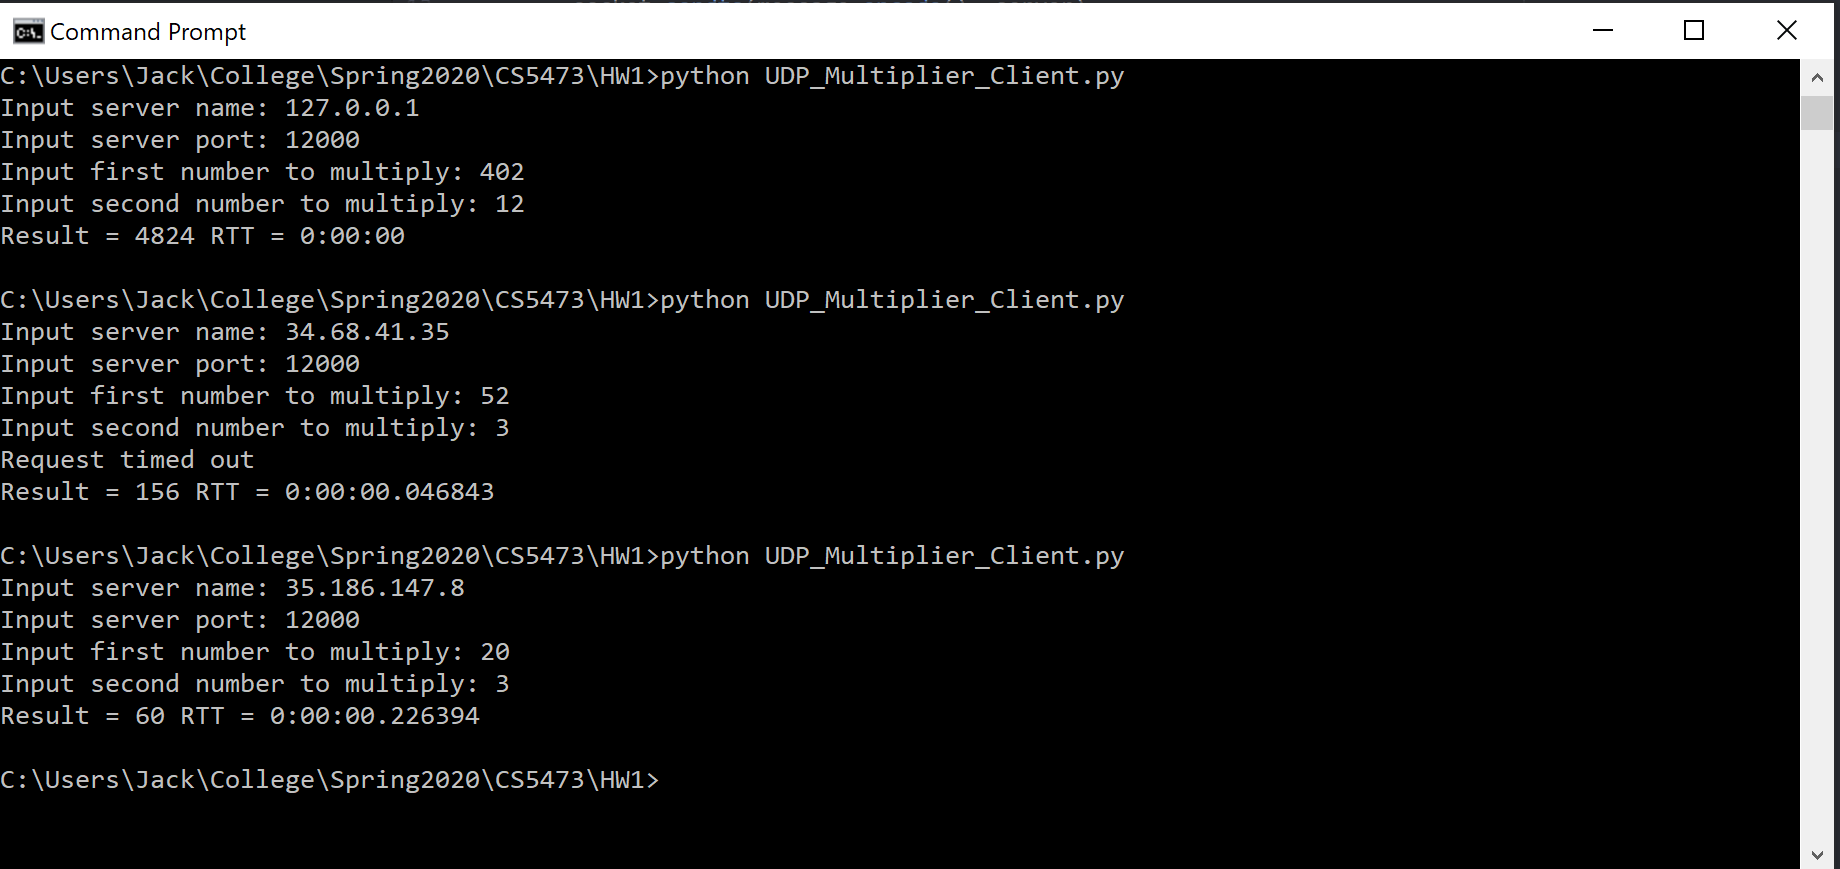
\includegraphics[width=\textwidth]{ping_comparison}


\section*{Problem 2}

delay $= ((56 $ bytes$ * (8 $ bits$/$bytes$)) / 64 $ kbps$) + 10 $ msec$ + ((56 $ bytes$ * (8 $ bits$/$byte$)) / 2 $ Mbps$) \\= 7 $ msec$ + 10 $ msec$ + 0.224 $ msec$	= 17.224$ msec


\section*{Problem3}

Second segment from A to B:

\begin{itemize}
	\item Sequence number = 207
	\item Source port number = 302
	\item Destination port number = 80
\end{itemize}
Acknowledgment of first arriving segment (if first sent arrives first):
\begin{itemize}
	\item Acknowledgment number = 127
	\item Source port number = 80
	\item Destination port number = 302
\end{itemize}
Acknowledgment of first arriving segment (if second arrives first):
\begin{itemize}
	\item Acknowledgment number = 201
\end{itemize}


\section*{Problem 4}

\begin{align}
\text{First two numbers:\ }
& 01010011\\
& 01100110\\
\text{Partial sum:\ }
& 10111001\\
\text{Add third number:\ }
& 01110100\\
\text{Sum:}
1 & 00101101\\
\text{Carryover:\ }
& 00101110\\
\text{Complement:\ }
& 11010001
\end{align}
1's complement = $11010001$

% --------------------------------------------------------------
%     You don't have to mess with anything below this line.
% --------------------------------------------------------------
 
\end{document}